\begin{figure}[p]
\centering
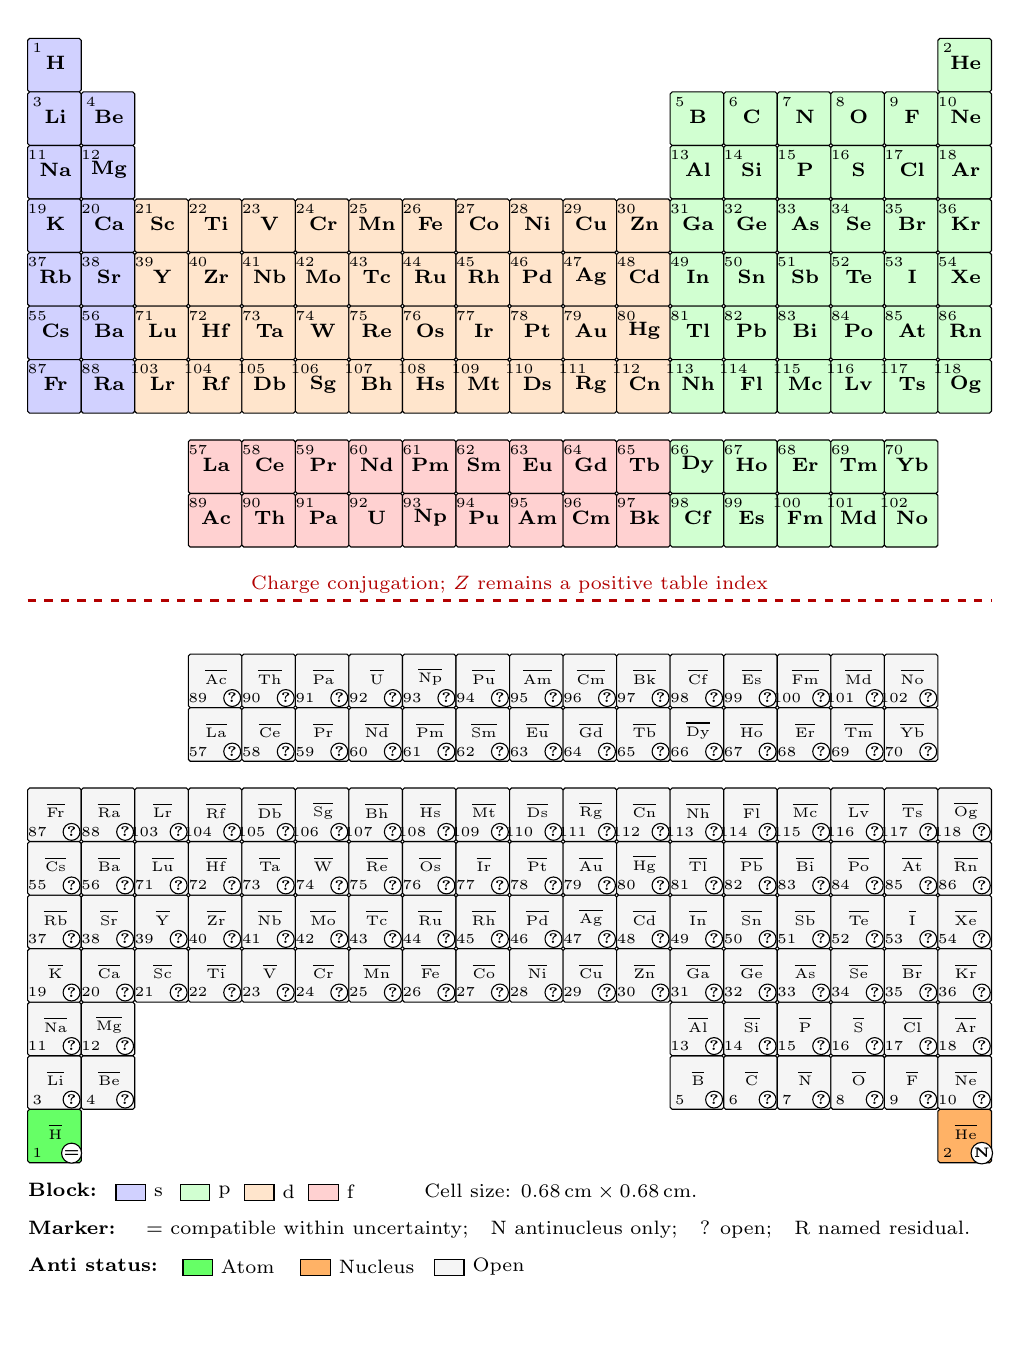
\begin{tikzpicture}[x=0.68cm, y=0.68cm, every node/.style={inner sep=0pt}]
\path[use as bounding box] (0,10.2) rectangle (18,-13.900000000000002);
\draw[fill=blue!18, draw=black, rounded corners=0.7pt] (0,10.0) rectangle (1,9.0);
\node at (0.52,9.54) {\scriptsize \textbf{H}};
\node at (0.18,9.82) {\tiny 1};
\draw[fill=green!18, draw=black, rounded corners=0.7pt] (17,10.0) rectangle (18,9.0);
\node at (17.52,9.54) {\scriptsize \textbf{He}};
\node at (17.18,9.82) {\tiny 2};
\draw[fill=blue!18, draw=black, rounded corners=0.7pt] (0,9.0) rectangle (1,8.0);
\node at (0.52,8.54) {\scriptsize \textbf{Li}};
\node at (0.18,8.82) {\tiny 3};
\draw[fill=blue!18, draw=black, rounded corners=0.7pt] (1,9.0) rectangle (2,8.0);
\node at (1.52,8.54) {\scriptsize \textbf{Be}};
\node at (1.18,8.82) {\tiny 4};
\draw[fill=green!18, draw=black, rounded corners=0.7pt] (12,9.0) rectangle (13,8.0);
\node at (12.52,8.54) {\scriptsize \textbf{B}};
\node at (12.18,8.82) {\tiny 5};
\draw[fill=green!18, draw=black, rounded corners=0.7pt] (13,9.0) rectangle (14,8.0);
\node at (13.52,8.54) {\scriptsize \textbf{C}};
\node at (13.18,8.82) {\tiny 6};
\draw[fill=green!18, draw=black, rounded corners=0.7pt] (14,9.0) rectangle (15,8.0);
\node at (14.52,8.54) {\scriptsize \textbf{N}};
\node at (14.18,8.82) {\tiny 7};
\draw[fill=green!18, draw=black, rounded corners=0.7pt] (15,9.0) rectangle (16,8.0);
\node at (15.52,8.54) {\scriptsize \textbf{O}};
\node at (15.18,8.82) {\tiny 8};
\draw[fill=green!18, draw=black, rounded corners=0.7pt] (16,9.0) rectangle (17,8.0);
\node at (16.52,8.54) {\scriptsize \textbf{F}};
\node at (16.18,8.82) {\tiny 9};
\draw[fill=green!18, draw=black, rounded corners=0.7pt] (17,9.0) rectangle (18,8.0);
\node at (17.52,8.54) {\scriptsize \textbf{Ne}};
\node at (17.18,8.82) {\tiny 10};
\draw[fill=blue!18, draw=black, rounded corners=0.7pt] (0,8.0) rectangle (1,7.0);
\node at (0.52,7.54) {\scriptsize \textbf{Na}};
\node at (0.18,7.82) {\tiny 11};
\draw[fill=blue!18, draw=black, rounded corners=0.7pt] (1,8.0) rectangle (2,7.0);
\node at (1.52,7.54) {\scriptsize \textbf{Mg}};
\node at (1.18,7.82) {\tiny 12};
\draw[fill=green!18, draw=black, rounded corners=0.7pt] (12,8.0) rectangle (13,7.0);
\node at (12.52,7.54) {\scriptsize \textbf{Al}};
\node at (12.18,7.82) {\tiny 13};
\draw[fill=green!18, draw=black, rounded corners=0.7pt] (13,8.0) rectangle (14,7.0);
\node at (13.52,7.54) {\scriptsize \textbf{Si}};
\node at (13.18,7.82) {\tiny 14};
\draw[fill=green!18, draw=black, rounded corners=0.7pt] (14,8.0) rectangle (15,7.0);
\node at (14.52,7.54) {\scriptsize \textbf{P}};
\node at (14.18,7.82) {\tiny 15};
\draw[fill=green!18, draw=black, rounded corners=0.7pt] (15,8.0) rectangle (16,7.0);
\node at (15.52,7.54) {\scriptsize \textbf{S}};
\node at (15.18,7.82) {\tiny 16};
\draw[fill=green!18, draw=black, rounded corners=0.7pt] (16,8.0) rectangle (17,7.0);
\node at (16.52,7.54) {\scriptsize \textbf{Cl}};
\node at (16.18,7.82) {\tiny 17};
\draw[fill=green!18, draw=black, rounded corners=0.7pt] (17,8.0) rectangle (18,7.0);
\node at (17.52,7.54) {\scriptsize \textbf{Ar}};
\node at (17.18,7.82) {\tiny 18};
\draw[fill=blue!18, draw=black, rounded corners=0.7pt] (0,7.0) rectangle (1,6.0);
\node at (0.52,6.54) {\scriptsize \textbf{K}};
\node at (0.18,6.82) {\tiny 19};
\draw[fill=blue!18, draw=black, rounded corners=0.7pt] (1,7.0) rectangle (2,6.0);
\node at (1.52,6.54) {\scriptsize \textbf{Ca}};
\node at (1.18,6.82) {\tiny 20};
\draw[fill=orange!20, draw=black, rounded corners=0.7pt] (2,7.0) rectangle (3,6.0);
\node at (2.52,6.54) {\scriptsize \textbf{Sc}};
\node at (2.18,6.82) {\tiny 21};
\draw[fill=orange!20, draw=black, rounded corners=0.7pt] (3,7.0) rectangle (4,6.0);
\node at (3.52,6.54) {\scriptsize \textbf{Ti}};
\node at (3.18,6.82) {\tiny 22};
\draw[fill=orange!20, draw=black, rounded corners=0.7pt] (4,7.0) rectangle (5,6.0);
\node at (4.52,6.54) {\scriptsize \textbf{V}};
\node at (4.18,6.82) {\tiny 23};
\draw[fill=orange!20, draw=black, rounded corners=0.7pt] (5,7.0) rectangle (6,6.0);
\node at (5.52,6.54) {\scriptsize \textbf{Cr}};
\node at (5.18,6.82) {\tiny 24};
\draw[fill=orange!20, draw=black, rounded corners=0.7pt] (6,7.0) rectangle (7,6.0);
\node at (6.52,6.54) {\scriptsize \textbf{Mn}};
\node at (6.18,6.82) {\tiny 25};
\draw[fill=orange!20, draw=black, rounded corners=0.7pt] (7,7.0) rectangle (8,6.0);
\node at (7.52,6.54) {\scriptsize \textbf{Fe}};
\node at (7.18,6.82) {\tiny 26};
\draw[fill=orange!20, draw=black, rounded corners=0.7pt] (8,7.0) rectangle (9,6.0);
\node at (8.52,6.54) {\scriptsize \textbf{Co}};
\node at (8.18,6.82) {\tiny 27};
\draw[fill=orange!20, draw=black, rounded corners=0.7pt] (9,7.0) rectangle (10,6.0);
\node at (9.52,6.54) {\scriptsize \textbf{Ni}};
\node at (9.18,6.82) {\tiny 28};
\draw[fill=orange!20, draw=black, rounded corners=0.7pt] (10,7.0) rectangle (11,6.0);
\node at (10.52,6.54) {\scriptsize \textbf{Cu}};
\node at (10.18,6.82) {\tiny 29};
\draw[fill=orange!20, draw=black, rounded corners=0.7pt] (11,7.0) rectangle (12,6.0);
\node at (11.52,6.54) {\scriptsize \textbf{Zn}};
\node at (11.18,6.82) {\tiny 30};
\draw[fill=green!18, draw=black, rounded corners=0.7pt] (12,7.0) rectangle (13,6.0);
\node at (12.52,6.54) {\scriptsize \textbf{Ga}};
\node at (12.18,6.82) {\tiny 31};
\draw[fill=green!18, draw=black, rounded corners=0.7pt] (13,7.0) rectangle (14,6.0);
\node at (13.52,6.54) {\scriptsize \textbf{Ge}};
\node at (13.18,6.82) {\tiny 32};
\draw[fill=green!18, draw=black, rounded corners=0.7pt] (14,7.0) rectangle (15,6.0);
\node at (14.52,6.54) {\scriptsize \textbf{As}};
\node at (14.18,6.82) {\tiny 33};
\draw[fill=green!18, draw=black, rounded corners=0.7pt] (15,7.0) rectangle (16,6.0);
\node at (15.52,6.54) {\scriptsize \textbf{Se}};
\node at (15.18,6.82) {\tiny 34};
\draw[fill=green!18, draw=black, rounded corners=0.7pt] (16,7.0) rectangle (17,6.0);
\node at (16.52,6.54) {\scriptsize \textbf{Br}};
\node at (16.18,6.82) {\tiny 35};
\draw[fill=green!18, draw=black, rounded corners=0.7pt] (17,7.0) rectangle (18,6.0);
\node at (17.52,6.54) {\scriptsize \textbf{Kr}};
\node at (17.18,6.82) {\tiny 36};
\draw[fill=blue!18, draw=black, rounded corners=0.7pt] (0,6.0) rectangle (1,5.0);
\node at (0.52,5.54) {\scriptsize \textbf{Rb}};
\node at (0.18,5.82) {\tiny 37};
\draw[fill=blue!18, draw=black, rounded corners=0.7pt] (1,6.0) rectangle (2,5.0);
\node at (1.52,5.54) {\scriptsize \textbf{Sr}};
\node at (1.18,5.82) {\tiny 38};
\draw[fill=orange!20, draw=black, rounded corners=0.7pt] (2,6.0) rectangle (3,5.0);
\node at (2.52,5.54) {\scriptsize \textbf{Y}};
\node at (2.18,5.82) {\tiny 39};
\draw[fill=orange!20, draw=black, rounded corners=0.7pt] (3,6.0) rectangle (4,5.0);
\node at (3.52,5.54) {\scriptsize \textbf{Zr}};
\node at (3.18,5.82) {\tiny 40};
\draw[fill=orange!20, draw=black, rounded corners=0.7pt] (4,6.0) rectangle (5,5.0);
\node at (4.52,5.54) {\scriptsize \textbf{Nb}};
\node at (4.18,5.82) {\tiny 41};
\draw[fill=orange!20, draw=black, rounded corners=0.7pt] (5,6.0) rectangle (6,5.0);
\node at (5.52,5.54) {\scriptsize \textbf{Mo}};
\node at (5.18,5.82) {\tiny 42};
\draw[fill=orange!20, draw=black, rounded corners=0.7pt] (6,6.0) rectangle (7,5.0);
\node at (6.52,5.54) {\scriptsize \textbf{Tc}};
\node at (6.18,5.82) {\tiny 43};
\draw[fill=orange!20, draw=black, rounded corners=0.7pt] (7,6.0) rectangle (8,5.0);
\node at (7.52,5.54) {\scriptsize \textbf{Ru}};
\node at (7.18,5.82) {\tiny 44};
\draw[fill=orange!20, draw=black, rounded corners=0.7pt] (8,6.0) rectangle (9,5.0);
\node at (8.52,5.54) {\scriptsize \textbf{Rh}};
\node at (8.18,5.82) {\tiny 45};
\draw[fill=orange!20, draw=black, rounded corners=0.7pt] (9,6.0) rectangle (10,5.0);
\node at (9.52,5.54) {\scriptsize \textbf{Pd}};
\node at (9.18,5.82) {\tiny 46};
\draw[fill=orange!20, draw=black, rounded corners=0.7pt] (10,6.0) rectangle (11,5.0);
\node at (10.52,5.54) {\scriptsize \textbf{Ag}};
\node at (10.18,5.82) {\tiny 47};
\draw[fill=orange!20, draw=black, rounded corners=0.7pt] (11,6.0) rectangle (12,5.0);
\node at (11.52,5.54) {\scriptsize \textbf{Cd}};
\node at (11.18,5.82) {\tiny 48};
\draw[fill=green!18, draw=black, rounded corners=0.7pt] (12,6.0) rectangle (13,5.0);
\node at (12.52,5.54) {\scriptsize \textbf{In}};
\node at (12.18,5.82) {\tiny 49};
\draw[fill=green!18, draw=black, rounded corners=0.7pt] (13,6.0) rectangle (14,5.0);
\node at (13.52,5.54) {\scriptsize \textbf{Sn}};
\node at (13.18,5.82) {\tiny 50};
\draw[fill=green!18, draw=black, rounded corners=0.7pt] (14,6.0) rectangle (15,5.0);
\node at (14.52,5.54) {\scriptsize \textbf{Sb}};
\node at (14.18,5.82) {\tiny 51};
\draw[fill=green!18, draw=black, rounded corners=0.7pt] (15,6.0) rectangle (16,5.0);
\node at (15.52,5.54) {\scriptsize \textbf{Te}};
\node at (15.18,5.82) {\tiny 52};
\draw[fill=green!18, draw=black, rounded corners=0.7pt] (16,6.0) rectangle (17,5.0);
\node at (16.52,5.54) {\scriptsize \textbf{I}};
\node at (16.18,5.82) {\tiny 53};
\draw[fill=green!18, draw=black, rounded corners=0.7pt] (17,6.0) rectangle (18,5.0);
\node at (17.52,5.54) {\scriptsize \textbf{Xe}};
\node at (17.18,5.82) {\tiny 54};
\draw[fill=blue!18, draw=black, rounded corners=0.7pt] (0,5.0) rectangle (1,4.0);
\node at (0.52,4.54) {\scriptsize \textbf{Cs}};
\node at (0.18,4.82) {\tiny 55};
\draw[fill=blue!18, draw=black, rounded corners=0.7pt] (1,5.0) rectangle (2,4.0);
\node at (1.52,4.54) {\scriptsize \textbf{Ba}};
\node at (1.18,4.82) {\tiny 56};
\draw[fill=orange!20, draw=black, rounded corners=0.7pt] (2,5.0) rectangle (3,4.0);
\node at (2.52,4.54) {\scriptsize \textbf{Lu}};
\node at (2.18,4.82) {\tiny 71};
\draw[fill=orange!20, draw=black, rounded corners=0.7pt] (3,5.0) rectangle (4,4.0);
\node at (3.52,4.54) {\scriptsize \textbf{Hf}};
\node at (3.18,4.82) {\tiny 72};
\draw[fill=orange!20, draw=black, rounded corners=0.7pt] (4,5.0) rectangle (5,4.0);
\node at (4.52,4.54) {\scriptsize \textbf{Ta}};
\node at (4.18,4.82) {\tiny 73};
\draw[fill=orange!20, draw=black, rounded corners=0.7pt] (5,5.0) rectangle (6,4.0);
\node at (5.52,4.54) {\scriptsize \textbf{W}};
\node at (5.18,4.82) {\tiny 74};
\draw[fill=orange!20, draw=black, rounded corners=0.7pt] (6,5.0) rectangle (7,4.0);
\node at (6.52,4.54) {\scriptsize \textbf{Re}};
\node at (6.18,4.82) {\tiny 75};
\draw[fill=orange!20, draw=black, rounded corners=0.7pt] (7,5.0) rectangle (8,4.0);
\node at (7.52,4.54) {\scriptsize \textbf{Os}};
\node at (7.18,4.82) {\tiny 76};
\draw[fill=orange!20, draw=black, rounded corners=0.7pt] (8,5.0) rectangle (9,4.0);
\node at (8.52,4.54) {\scriptsize \textbf{Ir}};
\node at (8.18,4.82) {\tiny 77};
\draw[fill=orange!20, draw=black, rounded corners=0.7pt] (9,5.0) rectangle (10,4.0);
\node at (9.52,4.54) {\scriptsize \textbf{Pt}};
\node at (9.18,4.82) {\tiny 78};
\draw[fill=orange!20, draw=black, rounded corners=0.7pt] (10,5.0) rectangle (11,4.0);
\node at (10.52,4.54) {\scriptsize \textbf{Au}};
\node at (10.18,4.82) {\tiny 79};
\draw[fill=orange!20, draw=black, rounded corners=0.7pt] (11,5.0) rectangle (12,4.0);
\node at (11.52,4.54) {\scriptsize \textbf{Hg}};
\node at (11.18,4.82) {\tiny 80};
\draw[fill=green!18, draw=black, rounded corners=0.7pt] (12,5.0) rectangle (13,4.0);
\node at (12.52,4.54) {\scriptsize \textbf{Tl}};
\node at (12.18,4.82) {\tiny 81};
\draw[fill=green!18, draw=black, rounded corners=0.7pt] (13,5.0) rectangle (14,4.0);
\node at (13.52,4.54) {\scriptsize \textbf{Pb}};
\node at (13.18,4.82) {\tiny 82};
\draw[fill=green!18, draw=black, rounded corners=0.7pt] (14,5.0) rectangle (15,4.0);
\node at (14.52,4.54) {\scriptsize \textbf{Bi}};
\node at (14.18,4.82) {\tiny 83};
\draw[fill=green!18, draw=black, rounded corners=0.7pt] (15,5.0) rectangle (16,4.0);
\node at (15.52,4.54) {\scriptsize \textbf{Po}};
\node at (15.18,4.82) {\tiny 84};
\draw[fill=green!18, draw=black, rounded corners=0.7pt] (16,5.0) rectangle (17,4.0);
\node at (16.52,4.54) {\scriptsize \textbf{At}};
\node at (16.18,4.82) {\tiny 85};
\draw[fill=green!18, draw=black, rounded corners=0.7pt] (17,5.0) rectangle (18,4.0);
\node at (17.52,4.54) {\scriptsize \textbf{Rn}};
\node at (17.18,4.82) {\tiny 86};
\draw[fill=blue!18, draw=black, rounded corners=0.7pt] (0,4.0) rectangle (1,3.0);
\node at (0.52,3.54) {\scriptsize \textbf{Fr}};
\node at (0.18,3.82) {\tiny 87};
\draw[fill=blue!18, draw=black, rounded corners=0.7pt] (1,4.0) rectangle (2,3.0);
\node at (1.52,3.54) {\scriptsize \textbf{Ra}};
\node at (1.18,3.82) {\tiny 88};
\draw[fill=orange!20, draw=black, rounded corners=0.7pt] (2,4.0) rectangle (3,3.0);
\node at (2.52,3.54) {\scriptsize \textbf{Lr}};
\node at (2.18,3.82) {\tiny 103};
\draw[fill=orange!20, draw=black, rounded corners=0.7pt] (3,4.0) rectangle (4,3.0);
\node at (3.52,3.54) {\scriptsize \textbf{Rf}};
\node at (3.18,3.82) {\tiny 104};
\draw[fill=orange!20, draw=black, rounded corners=0.7pt] (4,4.0) rectangle (5,3.0);
\node at (4.52,3.54) {\scriptsize \textbf{Db}};
\node at (4.18,3.82) {\tiny 105};
\draw[fill=orange!20, draw=black, rounded corners=0.7pt] (5,4.0) rectangle (6,3.0);
\node at (5.52,3.54) {\scriptsize \textbf{Sg}};
\node at (5.18,3.82) {\tiny 106};
\draw[fill=orange!20, draw=black, rounded corners=0.7pt] (6,4.0) rectangle (7,3.0);
\node at (6.52,3.54) {\scriptsize \textbf{Bh}};
\node at (6.18,3.82) {\tiny 107};
\draw[fill=orange!20, draw=black, rounded corners=0.7pt] (7,4.0) rectangle (8,3.0);
\node at (7.52,3.54) {\scriptsize \textbf{Hs}};
\node at (7.18,3.82) {\tiny 108};
\draw[fill=orange!20, draw=black, rounded corners=0.7pt] (8,4.0) rectangle (9,3.0);
\node at (8.52,3.54) {\scriptsize \textbf{Mt}};
\node at (8.18,3.82) {\tiny 109};
\draw[fill=orange!20, draw=black, rounded corners=0.7pt] (9,4.0) rectangle (10,3.0);
\node at (9.52,3.54) {\scriptsize \textbf{Ds}};
\node at (9.18,3.82) {\tiny 110};
\draw[fill=orange!20, draw=black, rounded corners=0.7pt] (10,4.0) rectangle (11,3.0);
\node at (10.52,3.54) {\scriptsize \textbf{Rg}};
\node at (10.18,3.82) {\tiny 111};
\draw[fill=orange!20, draw=black, rounded corners=0.7pt] (11,4.0) rectangle (12,3.0);
\node at (11.52,3.54) {\scriptsize \textbf{Cn}};
\node at (11.18,3.82) {\tiny 112};
\draw[fill=green!18, draw=black, rounded corners=0.7pt] (12,4.0) rectangle (13,3.0);
\node at (12.52,3.54) {\scriptsize \textbf{Nh}};
\node at (12.18,3.82) {\tiny 113};
\draw[fill=green!18, draw=black, rounded corners=0.7pt] (13,4.0) rectangle (14,3.0);
\node at (13.52,3.54) {\scriptsize \textbf{Fl}};
\node at (13.18,3.82) {\tiny 114};
\draw[fill=green!18, draw=black, rounded corners=0.7pt] (14,4.0) rectangle (15,3.0);
\node at (14.52,3.54) {\scriptsize \textbf{Mc}};
\node at (14.18,3.82) {\tiny 115};
\draw[fill=green!18, draw=black, rounded corners=0.7pt] (15,4.0) rectangle (16,3.0);
\node at (15.52,3.54) {\scriptsize \textbf{Lv}};
\node at (15.18,3.82) {\tiny 116};
\draw[fill=green!18, draw=black, rounded corners=0.7pt] (16,4.0) rectangle (17,3.0);
\node at (16.52,3.54) {\scriptsize \textbf{Ts}};
\node at (16.18,3.82) {\tiny 117};
\draw[fill=green!18, draw=black, rounded corners=0.7pt] (17,4.0) rectangle (18,3.0);
\node at (17.52,3.54) {\scriptsize \textbf{Og}};
\node at (17.18,3.82) {\tiny 118};
\draw[fill=red!18, draw=black, rounded corners=0.7pt] (3,2.5) rectangle (4,1.5);
\node at (3.52,2.04) {\scriptsize \textbf{La}};
\node at (3.18,2.32) {\tiny 57};
\draw[fill=red!18, draw=black, rounded corners=0.7pt] (4,2.5) rectangle (5,1.5);
\node at (4.52,2.04) {\scriptsize \textbf{Ce}};
\node at (4.18,2.32) {\tiny 58};
\draw[fill=red!18, draw=black, rounded corners=0.7pt] (5,2.5) rectangle (6,1.5);
\node at (5.52,2.04) {\scriptsize \textbf{Pr}};
\node at (5.18,2.32) {\tiny 59};
\draw[fill=red!18, draw=black, rounded corners=0.7pt] (6,2.5) rectangle (7,1.5);
\node at (6.52,2.04) {\scriptsize \textbf{Nd}};
\node at (6.18,2.32) {\tiny 60};
\draw[fill=red!18, draw=black, rounded corners=0.7pt] (7,2.5) rectangle (8,1.5);
\node at (7.52,2.04) {\scriptsize \textbf{Pm}};
\node at (7.18,2.32) {\tiny 61};
\draw[fill=red!18, draw=black, rounded corners=0.7pt] (8,2.5) rectangle (9,1.5);
\node at (8.52,2.04) {\scriptsize \textbf{Sm}};
\node at (8.18,2.32) {\tiny 62};
\draw[fill=red!18, draw=black, rounded corners=0.7pt] (9,2.5) rectangle (10,1.5);
\node at (9.52,2.04) {\scriptsize \textbf{Eu}};
\node at (9.18,2.32) {\tiny 63};
\draw[fill=red!18, draw=black, rounded corners=0.7pt] (10,2.5) rectangle (11,1.5);
\node at (10.52,2.04) {\scriptsize \textbf{Gd}};
\node at (10.18,2.32) {\tiny 64};
\draw[fill=red!18, draw=black, rounded corners=0.7pt] (11,2.5) rectangle (12,1.5);
\node at (11.52,2.04) {\scriptsize \textbf{Tb}};
\node at (11.18,2.32) {\tiny 65};
\draw[fill=green!18, draw=black, rounded corners=0.7pt] (12,2.5) rectangle (13,1.5);
\node at (12.52,2.04) {\scriptsize \textbf{Dy}};
\node at (12.18,2.32) {\tiny 66};
\draw[fill=green!18, draw=black, rounded corners=0.7pt] (13,2.5) rectangle (14,1.5);
\node at (13.52,2.04) {\scriptsize \textbf{Ho}};
\node at (13.18,2.32) {\tiny 67};
\draw[fill=green!18, draw=black, rounded corners=0.7pt] (14,2.5) rectangle (15,1.5);
\node at (14.52,2.04) {\scriptsize \textbf{Er}};
\node at (14.18,2.32) {\tiny 68};
\draw[fill=green!18, draw=black, rounded corners=0.7pt] (15,2.5) rectangle (16,1.5);
\node at (15.52,2.04) {\scriptsize \textbf{Tm}};
\node at (15.18,2.32) {\tiny 69};
\draw[fill=green!18, draw=black, rounded corners=0.7pt] (16,2.5) rectangle (17,1.5);
\node at (16.52,2.04) {\scriptsize \textbf{Yb}};
\node at (16.18,2.32) {\tiny 70};
\draw[fill=red!18, draw=black, rounded corners=0.7pt] (3,1.5) rectangle (4,0.5);
\node at (3.52,1.04) {\scriptsize \textbf{Ac}};
\node at (3.18,1.32) {\tiny 89};
\draw[fill=red!18, draw=black, rounded corners=0.7pt] (4,1.5) rectangle (5,0.5);
\node at (4.52,1.04) {\scriptsize \textbf{Th}};
\node at (4.18,1.32) {\tiny 90};
\draw[fill=red!18, draw=black, rounded corners=0.7pt] (5,1.5) rectangle (6,0.5);
\node at (5.52,1.04) {\scriptsize \textbf{Pa}};
\node at (5.18,1.32) {\tiny 91};
\draw[fill=red!18, draw=black, rounded corners=0.7pt] (6,1.5) rectangle (7,0.5);
\node at (6.52,1.04) {\scriptsize \textbf{U}};
\node at (6.18,1.32) {\tiny 92};
\draw[fill=red!18, draw=black, rounded corners=0.7pt] (7,1.5) rectangle (8,0.5);
\node at (7.52,1.04) {\scriptsize \textbf{Np}};
\node at (7.18,1.32) {\tiny 93};
\draw[fill=red!18, draw=black, rounded corners=0.7pt] (8,1.5) rectangle (9,0.5);
\node at (8.52,1.04) {\scriptsize \textbf{Pu}};
\node at (8.18,1.32) {\tiny 94};
\draw[fill=red!18, draw=black, rounded corners=0.7pt] (9,1.5) rectangle (10,0.5);
\node at (9.52,1.04) {\scriptsize \textbf{Am}};
\node at (9.18,1.32) {\tiny 95};
\draw[fill=red!18, draw=black, rounded corners=0.7pt] (10,1.5) rectangle (11,0.5);
\node at (10.52,1.04) {\scriptsize \textbf{Cm}};
\node at (10.18,1.32) {\tiny 96};
\draw[fill=red!18, draw=black, rounded corners=0.7pt] (11,1.5) rectangle (12,0.5);
\node at (11.52,1.04) {\scriptsize \textbf{Bk}};
\node at (11.18,1.32) {\tiny 97};
\draw[fill=green!18, draw=black, rounded corners=0.7pt] (12,1.5) rectangle (13,0.5);
\node at (12.52,1.04) {\scriptsize \textbf{Cf}};
\node at (12.18,1.32) {\tiny 98};
\draw[fill=green!18, draw=black, rounded corners=0.7pt] (13,1.5) rectangle (14,0.5);
\node at (13.52,1.04) {\scriptsize \textbf{Es}};
\node at (13.18,1.32) {\tiny 99};
\draw[fill=green!18, draw=black, rounded corners=0.7pt] (14,1.5) rectangle (15,0.5);
\node at (14.52,1.04) {\scriptsize \textbf{Fm}};
\node at (14.18,1.32) {\tiny 100};
\draw[fill=green!18, draw=black, rounded corners=0.7pt] (15,1.5) rectangle (16,0.5);
\node at (15.52,1.04) {\scriptsize \textbf{Md}};
\node at (15.18,1.32) {\tiny 101};
\draw[fill=green!18, draw=black, rounded corners=0.7pt] (16,1.5) rectangle (17,0.5);
\node at (16.52,1.04) {\scriptsize \textbf{No}};
\node at (16.18,1.32) {\tiny 102};
\draw[line width=1.2pt, dashed, red!70!black] (0,-0.5) -- (18,-0.5) node[midway, above=2pt, text=red!70!black] {\scriptsize Charge conjugation; $Z$ remains a positive table index};
\draw[fill=green!60, draw=black, rounded corners=0.7pt] (0,-10.0) rectangle (1,-11.0);
\node at (0.52,-10.42) {\tiny \textbf{$\overline{\mathrm{H}}$}};
\node at (0.18,-10.82) {\tiny 1};
\node[fill=white, draw=black, circle, inner sep=0.4pt] at (0.82,-10.82) {\tiny \textbf{=}};
\draw[fill=orange!60, draw=black, rounded corners=0.7pt] (17,-10.0) rectangle (18,-11.0);
\node at (17.52,-10.42) {\tiny \textbf{$\overline{\mathrm{He}}$}};
\node at (17.18,-10.82) {\tiny 2};
\node[fill=white, draw=black, circle, inner sep=0.4pt] at (17.82,-10.82) {\tiny \textbf{N}};
\draw[fill=gray!8, draw=black, rounded corners=0.7pt] (0,-9.0) rectangle (1,-10.0);
\node at (0.52,-9.42) {\tiny \textbf{$\overline{\mathrm{Li}}$}};
\node at (0.18,-9.82) {\tiny 3};
\node[fill=white, draw=black, circle, inner sep=0.4pt] at (0.82,-9.82) {\tiny \textbf{?}};
\draw[fill=gray!8, draw=black, rounded corners=0.7pt] (1,-9.0) rectangle (2,-10.0);
\node at (1.52,-9.42) {\tiny \textbf{$\overline{\mathrm{Be}}$}};
\node at (1.18,-9.82) {\tiny 4};
\node[fill=white, draw=black, circle, inner sep=0.4pt] at (1.8199999999999998,-9.82) {\tiny \textbf{?}};
\draw[fill=gray!8, draw=black, rounded corners=0.7pt] (12,-9.0) rectangle (13,-10.0);
\node at (12.52,-9.42) {\tiny \textbf{$\overline{\mathrm{B}}$}};
\node at (12.18,-9.82) {\tiny 5};
\node[fill=white, draw=black, circle, inner sep=0.4pt] at (12.82,-9.82) {\tiny \textbf{?}};
\draw[fill=gray!8, draw=black, rounded corners=0.7pt] (13,-9.0) rectangle (14,-10.0);
\node at (13.52,-9.42) {\tiny \textbf{$\overline{\mathrm{C}}$}};
\node at (13.18,-9.82) {\tiny 6};
\node[fill=white, draw=black, circle, inner sep=0.4pt] at (13.82,-9.82) {\tiny \textbf{?}};
\draw[fill=gray!8, draw=black, rounded corners=0.7pt] (14,-9.0) rectangle (15,-10.0);
\node at (14.52,-9.42) {\tiny \textbf{$\overline{\mathrm{N}}$}};
\node at (14.18,-9.82) {\tiny 7};
\node[fill=white, draw=black, circle, inner sep=0.4pt] at (14.82,-9.82) {\tiny \textbf{?}};
\draw[fill=gray!8, draw=black, rounded corners=0.7pt] (15,-9.0) rectangle (16,-10.0);
\node at (15.52,-9.42) {\tiny \textbf{$\overline{\mathrm{O}}$}};
\node at (15.18,-9.82) {\tiny 8};
\node[fill=white, draw=black, circle, inner sep=0.4pt] at (15.82,-9.82) {\tiny \textbf{?}};
\draw[fill=gray!8, draw=black, rounded corners=0.7pt] (16,-9.0) rectangle (17,-10.0);
\node at (16.52,-9.42) {\tiny \textbf{$\overline{\mathrm{F}}$}};
\node at (16.18,-9.82) {\tiny 9};
\node[fill=white, draw=black, circle, inner sep=0.4pt] at (16.82,-9.82) {\tiny \textbf{?}};
\draw[fill=gray!8, draw=black, rounded corners=0.7pt] (17,-9.0) rectangle (18,-10.0);
\node at (17.52,-9.42) {\tiny \textbf{$\overline{\mathrm{Ne}}$}};
\node at (17.18,-9.82) {\tiny 10};
\node[fill=white, draw=black, circle, inner sep=0.4pt] at (17.82,-9.82) {\tiny \textbf{?}};
\draw[fill=gray!8, draw=black, rounded corners=0.7pt] (0,-8.0) rectangle (1,-9.0);
\node at (0.52,-8.42) {\tiny \textbf{$\overline{\mathrm{Na}}$}};
\node at (0.18,-8.82) {\tiny 11};
\node[fill=white, draw=black, circle, inner sep=0.4pt] at (0.82,-8.82) {\tiny \textbf{?}};
\draw[fill=gray!8, draw=black, rounded corners=0.7pt] (1,-8.0) rectangle (2,-9.0);
\node at (1.52,-8.42) {\tiny \textbf{$\overline{\mathrm{Mg}}$}};
\node at (1.18,-8.82) {\tiny 12};
\node[fill=white, draw=black, circle, inner sep=0.4pt] at (1.8199999999999998,-8.82) {\tiny \textbf{?}};
\draw[fill=gray!8, draw=black, rounded corners=0.7pt] (12,-8.0) rectangle (13,-9.0);
\node at (12.52,-8.42) {\tiny \textbf{$\overline{\mathrm{Al}}$}};
\node at (12.18,-8.82) {\tiny 13};
\node[fill=white, draw=black, circle, inner sep=0.4pt] at (12.82,-8.82) {\tiny \textbf{?}};
\draw[fill=gray!8, draw=black, rounded corners=0.7pt] (13,-8.0) rectangle (14,-9.0);
\node at (13.52,-8.42) {\tiny \textbf{$\overline{\mathrm{Si}}$}};
\node at (13.18,-8.82) {\tiny 14};
\node[fill=white, draw=black, circle, inner sep=0.4pt] at (13.82,-8.82) {\tiny \textbf{?}};
\draw[fill=gray!8, draw=black, rounded corners=0.7pt] (14,-8.0) rectangle (15,-9.0);
\node at (14.52,-8.42) {\tiny \textbf{$\overline{\mathrm{P}}$}};
\node at (14.18,-8.82) {\tiny 15};
\node[fill=white, draw=black, circle, inner sep=0.4pt] at (14.82,-8.82) {\tiny \textbf{?}};
\draw[fill=gray!8, draw=black, rounded corners=0.7pt] (15,-8.0) rectangle (16,-9.0);
\node at (15.52,-8.42) {\tiny \textbf{$\overline{\mathrm{S}}$}};
\node at (15.18,-8.82) {\tiny 16};
\node[fill=white, draw=black, circle, inner sep=0.4pt] at (15.82,-8.82) {\tiny \textbf{?}};
\draw[fill=gray!8, draw=black, rounded corners=0.7pt] (16,-8.0) rectangle (17,-9.0);
\node at (16.52,-8.42) {\tiny \textbf{$\overline{\mathrm{Cl}}$}};
\node at (16.18,-8.82) {\tiny 17};
\node[fill=white, draw=black, circle, inner sep=0.4pt] at (16.82,-8.82) {\tiny \textbf{?}};
\draw[fill=gray!8, draw=black, rounded corners=0.7pt] (17,-8.0) rectangle (18,-9.0);
\node at (17.52,-8.42) {\tiny \textbf{$\overline{\mathrm{Ar}}$}};
\node at (17.18,-8.82) {\tiny 18};
\node[fill=white, draw=black, circle, inner sep=0.4pt] at (17.82,-8.82) {\tiny \textbf{?}};
\draw[fill=gray!8, draw=black, rounded corners=0.7pt] (0,-7.0) rectangle (1,-8.0);
\node at (0.52,-7.42) {\tiny \textbf{$\overline{\mathrm{K}}$}};
\node at (0.18,-7.82) {\tiny 19};
\node[fill=white, draw=black, circle, inner sep=0.4pt] at (0.82,-7.82) {\tiny \textbf{?}};
\draw[fill=gray!8, draw=black, rounded corners=0.7pt] (1,-7.0) rectangle (2,-8.0);
\node at (1.52,-7.42) {\tiny \textbf{$\overline{\mathrm{Ca}}$}};
\node at (1.18,-7.82) {\tiny 20};
\node[fill=white, draw=black, circle, inner sep=0.4pt] at (1.8199999999999998,-7.82) {\tiny \textbf{?}};
\draw[fill=gray!8, draw=black, rounded corners=0.7pt] (2,-7.0) rectangle (3,-8.0);
\node at (2.52,-7.42) {\tiny \textbf{$\overline{\mathrm{Sc}}$}};
\node at (2.18,-7.82) {\tiny 21};
\node[fill=white, draw=black, circle, inner sep=0.4pt] at (2.82,-7.82) {\tiny \textbf{?}};
\draw[fill=gray!8, draw=black, rounded corners=0.7pt] (3,-7.0) rectangle (4,-8.0);
\node at (3.52,-7.42) {\tiny \textbf{$\overline{\mathrm{Ti}}$}};
\node at (3.18,-7.82) {\tiny 22};
\node[fill=white, draw=black, circle, inner sep=0.4pt] at (3.82,-7.82) {\tiny \textbf{?}};
\draw[fill=gray!8, draw=black, rounded corners=0.7pt] (4,-7.0) rectangle (5,-8.0);
\node at (4.52,-7.42) {\tiny \textbf{$\overline{\mathrm{V}}$}};
\node at (4.18,-7.82) {\tiny 23};
\node[fill=white, draw=black, circle, inner sep=0.4pt] at (4.82,-7.82) {\tiny \textbf{?}};
\draw[fill=gray!8, draw=black, rounded corners=0.7pt] (5,-7.0) rectangle (6,-8.0);
\node at (5.52,-7.42) {\tiny \textbf{$\overline{\mathrm{Cr}}$}};
\node at (5.18,-7.82) {\tiny 24};
\node[fill=white, draw=black, circle, inner sep=0.4pt] at (5.82,-7.82) {\tiny \textbf{?}};
\draw[fill=gray!8, draw=black, rounded corners=0.7pt] (6,-7.0) rectangle (7,-8.0);
\node at (6.52,-7.42) {\tiny \textbf{$\overline{\mathrm{Mn}}$}};
\node at (6.18,-7.82) {\tiny 25};
\node[fill=white, draw=black, circle, inner sep=0.4pt] at (6.82,-7.82) {\tiny \textbf{?}};
\draw[fill=gray!8, draw=black, rounded corners=0.7pt] (7,-7.0) rectangle (8,-8.0);
\node at (7.52,-7.42) {\tiny \textbf{$\overline{\mathrm{Fe}}$}};
\node at (7.18,-7.82) {\tiny 26};
\node[fill=white, draw=black, circle, inner sep=0.4pt] at (7.82,-7.82) {\tiny \textbf{?}};
\draw[fill=gray!8, draw=black, rounded corners=0.7pt] (8,-7.0) rectangle (9,-8.0);
\node at (8.52,-7.42) {\tiny \textbf{$\overline{\mathrm{Co}}$}};
\node at (8.18,-7.82) {\tiny 27};
\node[fill=white, draw=black, circle, inner sep=0.4pt] at (8.82,-7.82) {\tiny \textbf{?}};
\draw[fill=gray!8, draw=black, rounded corners=0.7pt] (9,-7.0) rectangle (10,-8.0);
\node at (9.52,-7.42) {\tiny \textbf{$\overline{\mathrm{Ni}}$}};
\node at (9.18,-7.82) {\tiny 28};
\node[fill=white, draw=black, circle, inner sep=0.4pt] at (9.82,-7.82) {\tiny \textbf{?}};
\draw[fill=gray!8, draw=black, rounded corners=0.7pt] (10,-7.0) rectangle (11,-8.0);
\node at (10.52,-7.42) {\tiny \textbf{$\overline{\mathrm{Cu}}$}};
\node at (10.18,-7.82) {\tiny 29};
\node[fill=white, draw=black, circle, inner sep=0.4pt] at (10.82,-7.82) {\tiny \textbf{?}};
\draw[fill=gray!8, draw=black, rounded corners=0.7pt] (11,-7.0) rectangle (12,-8.0);
\node at (11.52,-7.42) {\tiny \textbf{$\overline{\mathrm{Zn}}$}};
\node at (11.18,-7.82) {\tiny 30};
\node[fill=white, draw=black, circle, inner sep=0.4pt] at (11.82,-7.82) {\tiny \textbf{?}};
\draw[fill=gray!8, draw=black, rounded corners=0.7pt] (12,-7.0) rectangle (13,-8.0);
\node at (12.52,-7.42) {\tiny \textbf{$\overline{\mathrm{Ga}}$}};
\node at (12.18,-7.82) {\tiny 31};
\node[fill=white, draw=black, circle, inner sep=0.4pt] at (12.82,-7.82) {\tiny \textbf{?}};
\draw[fill=gray!8, draw=black, rounded corners=0.7pt] (13,-7.0) rectangle (14,-8.0);
\node at (13.52,-7.42) {\tiny \textbf{$\overline{\mathrm{Ge}}$}};
\node at (13.18,-7.82) {\tiny 32};
\node[fill=white, draw=black, circle, inner sep=0.4pt] at (13.82,-7.82) {\tiny \textbf{?}};
\draw[fill=gray!8, draw=black, rounded corners=0.7pt] (14,-7.0) rectangle (15,-8.0);
\node at (14.52,-7.42) {\tiny \textbf{$\overline{\mathrm{As}}$}};
\node at (14.18,-7.82) {\tiny 33};
\node[fill=white, draw=black, circle, inner sep=0.4pt] at (14.82,-7.82) {\tiny \textbf{?}};
\draw[fill=gray!8, draw=black, rounded corners=0.7pt] (15,-7.0) rectangle (16,-8.0);
\node at (15.52,-7.42) {\tiny \textbf{$\overline{\mathrm{Se}}$}};
\node at (15.18,-7.82) {\tiny 34};
\node[fill=white, draw=black, circle, inner sep=0.4pt] at (15.82,-7.82) {\tiny \textbf{?}};
\draw[fill=gray!8, draw=black, rounded corners=0.7pt] (16,-7.0) rectangle (17,-8.0);
\node at (16.52,-7.42) {\tiny \textbf{$\overline{\mathrm{Br}}$}};
\node at (16.18,-7.82) {\tiny 35};
\node[fill=white, draw=black, circle, inner sep=0.4pt] at (16.82,-7.82) {\tiny \textbf{?}};
\draw[fill=gray!8, draw=black, rounded corners=0.7pt] (17,-7.0) rectangle (18,-8.0);
\node at (17.52,-7.42) {\tiny \textbf{$\overline{\mathrm{Kr}}$}};
\node at (17.18,-7.82) {\tiny 36};
\node[fill=white, draw=black, circle, inner sep=0.4pt] at (17.82,-7.82) {\tiny \textbf{?}};
\draw[fill=gray!8, draw=black, rounded corners=0.7pt] (0,-6.0) rectangle (1,-7.0);
\node at (0.52,-6.42) {\tiny \textbf{$\overline{\mathrm{Rb}}$}};
\node at (0.18,-6.82) {\tiny 37};
\node[fill=white, draw=black, circle, inner sep=0.4pt] at (0.82,-6.82) {\tiny \textbf{?}};
\draw[fill=gray!8, draw=black, rounded corners=0.7pt] (1,-6.0) rectangle (2,-7.0);
\node at (1.52,-6.42) {\tiny \textbf{$\overline{\mathrm{Sr}}$}};
\node at (1.18,-6.82) {\tiny 38};
\node[fill=white, draw=black, circle, inner sep=0.4pt] at (1.8199999999999998,-6.82) {\tiny \textbf{?}};
\draw[fill=gray!8, draw=black, rounded corners=0.7pt] (2,-6.0) rectangle (3,-7.0);
\node at (2.52,-6.42) {\tiny \textbf{$\overline{\mathrm{Y}}$}};
\node at (2.18,-6.82) {\tiny 39};
\node[fill=white, draw=black, circle, inner sep=0.4pt] at (2.82,-6.82) {\tiny \textbf{?}};
\draw[fill=gray!8, draw=black, rounded corners=0.7pt] (3,-6.0) rectangle (4,-7.0);
\node at (3.52,-6.42) {\tiny \textbf{$\overline{\mathrm{Zr}}$}};
\node at (3.18,-6.82) {\tiny 40};
\node[fill=white, draw=black, circle, inner sep=0.4pt] at (3.82,-6.82) {\tiny \textbf{?}};
\draw[fill=gray!8, draw=black, rounded corners=0.7pt] (4,-6.0) rectangle (5,-7.0);
\node at (4.52,-6.42) {\tiny \textbf{$\overline{\mathrm{Nb}}$}};
\node at (4.18,-6.82) {\tiny 41};
\node[fill=white, draw=black, circle, inner sep=0.4pt] at (4.82,-6.82) {\tiny \textbf{?}};
\draw[fill=gray!8, draw=black, rounded corners=0.7pt] (5,-6.0) rectangle (6,-7.0);
\node at (5.52,-6.42) {\tiny \textbf{$\overline{\mathrm{Mo}}$}};
\node at (5.18,-6.82) {\tiny 42};
\node[fill=white, draw=black, circle, inner sep=0.4pt] at (5.82,-6.82) {\tiny \textbf{?}};
\draw[fill=gray!8, draw=black, rounded corners=0.7pt] (6,-6.0) rectangle (7,-7.0);
\node at (6.52,-6.42) {\tiny \textbf{$\overline{\mathrm{Tc}}$}};
\node at (6.18,-6.82) {\tiny 43};
\node[fill=white, draw=black, circle, inner sep=0.4pt] at (6.82,-6.82) {\tiny \textbf{?}};
\draw[fill=gray!8, draw=black, rounded corners=0.7pt] (7,-6.0) rectangle (8,-7.0);
\node at (7.52,-6.42) {\tiny \textbf{$\overline{\mathrm{Ru}}$}};
\node at (7.18,-6.82) {\tiny 44};
\node[fill=white, draw=black, circle, inner sep=0.4pt] at (7.82,-6.82) {\tiny \textbf{?}};
\draw[fill=gray!8, draw=black, rounded corners=0.7pt] (8,-6.0) rectangle (9,-7.0);
\node at (8.52,-6.42) {\tiny \textbf{$\overline{\mathrm{Rh}}$}};
\node at (8.18,-6.82) {\tiny 45};
\node[fill=white, draw=black, circle, inner sep=0.4pt] at (8.82,-6.82) {\tiny \textbf{?}};
\draw[fill=gray!8, draw=black, rounded corners=0.7pt] (9,-6.0) rectangle (10,-7.0);
\node at (9.52,-6.42) {\tiny \textbf{$\overline{\mathrm{Pd}}$}};
\node at (9.18,-6.82) {\tiny 46};
\node[fill=white, draw=black, circle, inner sep=0.4pt] at (9.82,-6.82) {\tiny \textbf{?}};
\draw[fill=gray!8, draw=black, rounded corners=0.7pt] (10,-6.0) rectangle (11,-7.0);
\node at (10.52,-6.42) {\tiny \textbf{$\overline{\mathrm{Ag}}$}};
\node at (10.18,-6.82) {\tiny 47};
\node[fill=white, draw=black, circle, inner sep=0.4pt] at (10.82,-6.82) {\tiny \textbf{?}};
\draw[fill=gray!8, draw=black, rounded corners=0.7pt] (11,-6.0) rectangle (12,-7.0);
\node at (11.52,-6.42) {\tiny \textbf{$\overline{\mathrm{Cd}}$}};
\node at (11.18,-6.82) {\tiny 48};
\node[fill=white, draw=black, circle, inner sep=0.4pt] at (11.82,-6.82) {\tiny \textbf{?}};
\draw[fill=gray!8, draw=black, rounded corners=0.7pt] (12,-6.0) rectangle (13,-7.0);
\node at (12.52,-6.42) {\tiny \textbf{$\overline{\mathrm{In}}$}};
\node at (12.18,-6.82) {\tiny 49};
\node[fill=white, draw=black, circle, inner sep=0.4pt] at (12.82,-6.82) {\tiny \textbf{?}};
\draw[fill=gray!8, draw=black, rounded corners=0.7pt] (13,-6.0) rectangle (14,-7.0);
\node at (13.52,-6.42) {\tiny \textbf{$\overline{\mathrm{Sn}}$}};
\node at (13.18,-6.82) {\tiny 50};
\node[fill=white, draw=black, circle, inner sep=0.4pt] at (13.82,-6.82) {\tiny \textbf{?}};
\draw[fill=gray!8, draw=black, rounded corners=0.7pt] (14,-6.0) rectangle (15,-7.0);
\node at (14.52,-6.42) {\tiny \textbf{$\overline{\mathrm{Sb}}$}};
\node at (14.18,-6.82) {\tiny 51};
\node[fill=white, draw=black, circle, inner sep=0.4pt] at (14.82,-6.82) {\tiny \textbf{?}};
\draw[fill=gray!8, draw=black, rounded corners=0.7pt] (15,-6.0) rectangle (16,-7.0);
\node at (15.52,-6.42) {\tiny \textbf{$\overline{\mathrm{Te}}$}};
\node at (15.18,-6.82) {\tiny 52};
\node[fill=white, draw=black, circle, inner sep=0.4pt] at (15.82,-6.82) {\tiny \textbf{?}};
\draw[fill=gray!8, draw=black, rounded corners=0.7pt] (16,-6.0) rectangle (17,-7.0);
\node at (16.52,-6.42) {\tiny \textbf{$\overline{\mathrm{I}}$}};
\node at (16.18,-6.82) {\tiny 53};
\node[fill=white, draw=black, circle, inner sep=0.4pt] at (16.82,-6.82) {\tiny \textbf{?}};
\draw[fill=gray!8, draw=black, rounded corners=0.7pt] (17,-6.0) rectangle (18,-7.0);
\node at (17.52,-6.42) {\tiny \textbf{$\overline{\mathrm{Xe}}$}};
\node at (17.18,-6.82) {\tiny 54};
\node[fill=white, draw=black, circle, inner sep=0.4pt] at (17.82,-6.82) {\tiny \textbf{?}};
\draw[fill=gray!8, draw=black, rounded corners=0.7pt] (0,-5.0) rectangle (1,-6.0);
\node at (0.52,-5.42) {\tiny \textbf{$\overline{\mathrm{Cs}}$}};
\node at (0.18,-5.82) {\tiny 55};
\node[fill=white, draw=black, circle, inner sep=0.4pt] at (0.82,-5.82) {\tiny \textbf{?}};
\draw[fill=gray!8, draw=black, rounded corners=0.7pt] (1,-5.0) rectangle (2,-6.0);
\node at (1.52,-5.42) {\tiny \textbf{$\overline{\mathrm{Ba}}$}};
\node at (1.18,-5.82) {\tiny 56};
\node[fill=white, draw=black, circle, inner sep=0.4pt] at (1.8199999999999998,-5.82) {\tiny \textbf{?}};
\draw[fill=gray!8, draw=black, rounded corners=0.7pt] (2,-5.0) rectangle (3,-6.0);
\node at (2.52,-5.42) {\tiny \textbf{$\overline{\mathrm{Lu}}$}};
\node at (2.18,-5.82) {\tiny 71};
\node[fill=white, draw=black, circle, inner sep=0.4pt] at (2.82,-5.82) {\tiny \textbf{?}};
\draw[fill=gray!8, draw=black, rounded corners=0.7pt] (3,-5.0) rectangle (4,-6.0);
\node at (3.52,-5.42) {\tiny \textbf{$\overline{\mathrm{Hf}}$}};
\node at (3.18,-5.82) {\tiny 72};
\node[fill=white, draw=black, circle, inner sep=0.4pt] at (3.82,-5.82) {\tiny \textbf{?}};
\draw[fill=gray!8, draw=black, rounded corners=0.7pt] (4,-5.0) rectangle (5,-6.0);
\node at (4.52,-5.42) {\tiny \textbf{$\overline{\mathrm{Ta}}$}};
\node at (4.18,-5.82) {\tiny 73};
\node[fill=white, draw=black, circle, inner sep=0.4pt] at (4.82,-5.82) {\tiny \textbf{?}};
\draw[fill=gray!8, draw=black, rounded corners=0.7pt] (5,-5.0) rectangle (6,-6.0);
\node at (5.52,-5.42) {\tiny \textbf{$\overline{\mathrm{W}}$}};
\node at (5.18,-5.82) {\tiny 74};
\node[fill=white, draw=black, circle, inner sep=0.4pt] at (5.82,-5.82) {\tiny \textbf{?}};
\draw[fill=gray!8, draw=black, rounded corners=0.7pt] (6,-5.0) rectangle (7,-6.0);
\node at (6.52,-5.42) {\tiny \textbf{$\overline{\mathrm{Re}}$}};
\node at (6.18,-5.82) {\tiny 75};
\node[fill=white, draw=black, circle, inner sep=0.4pt] at (6.82,-5.82) {\tiny \textbf{?}};
\draw[fill=gray!8, draw=black, rounded corners=0.7pt] (7,-5.0) rectangle (8,-6.0);
\node at (7.52,-5.42) {\tiny \textbf{$\overline{\mathrm{Os}}$}};
\node at (7.18,-5.82) {\tiny 76};
\node[fill=white, draw=black, circle, inner sep=0.4pt] at (7.82,-5.82) {\tiny \textbf{?}};
\draw[fill=gray!8, draw=black, rounded corners=0.7pt] (8,-5.0) rectangle (9,-6.0);
\node at (8.52,-5.42) {\tiny \textbf{$\overline{\mathrm{Ir}}$}};
\node at (8.18,-5.82) {\tiny 77};
\node[fill=white, draw=black, circle, inner sep=0.4pt] at (8.82,-5.82) {\tiny \textbf{?}};
\draw[fill=gray!8, draw=black, rounded corners=0.7pt] (9,-5.0) rectangle (10,-6.0);
\node at (9.52,-5.42) {\tiny \textbf{$\overline{\mathrm{Pt}}$}};
\node at (9.18,-5.82) {\tiny 78};
\node[fill=white, draw=black, circle, inner sep=0.4pt] at (9.82,-5.82) {\tiny \textbf{?}};
\draw[fill=gray!8, draw=black, rounded corners=0.7pt] (10,-5.0) rectangle (11,-6.0);
\node at (10.52,-5.42) {\tiny \textbf{$\overline{\mathrm{Au}}$}};
\node at (10.18,-5.82) {\tiny 79};
\node[fill=white, draw=black, circle, inner sep=0.4pt] at (10.82,-5.82) {\tiny \textbf{?}};
\draw[fill=gray!8, draw=black, rounded corners=0.7pt] (11,-5.0) rectangle (12,-6.0);
\node at (11.52,-5.42) {\tiny \textbf{$\overline{\mathrm{Hg}}$}};
\node at (11.18,-5.82) {\tiny 80};
\node[fill=white, draw=black, circle, inner sep=0.4pt] at (11.82,-5.82) {\tiny \textbf{?}};
\draw[fill=gray!8, draw=black, rounded corners=0.7pt] (12,-5.0) rectangle (13,-6.0);
\node at (12.52,-5.42) {\tiny \textbf{$\overline{\mathrm{Tl}}$}};
\node at (12.18,-5.82) {\tiny 81};
\node[fill=white, draw=black, circle, inner sep=0.4pt] at (12.82,-5.82) {\tiny \textbf{?}};
\draw[fill=gray!8, draw=black, rounded corners=0.7pt] (13,-5.0) rectangle (14,-6.0);
\node at (13.52,-5.42) {\tiny \textbf{$\overline{\mathrm{Pb}}$}};
\node at (13.18,-5.82) {\tiny 82};
\node[fill=white, draw=black, circle, inner sep=0.4pt] at (13.82,-5.82) {\tiny \textbf{?}};
\draw[fill=gray!8, draw=black, rounded corners=0.7pt] (14,-5.0) rectangle (15,-6.0);
\node at (14.52,-5.42) {\tiny \textbf{$\overline{\mathrm{Bi}}$}};
\node at (14.18,-5.82) {\tiny 83};
\node[fill=white, draw=black, circle, inner sep=0.4pt] at (14.82,-5.82) {\tiny \textbf{?}};
\draw[fill=gray!8, draw=black, rounded corners=0.7pt] (15,-5.0) rectangle (16,-6.0);
\node at (15.52,-5.42) {\tiny \textbf{$\overline{\mathrm{Po}}$}};
\node at (15.18,-5.82) {\tiny 84};
\node[fill=white, draw=black, circle, inner sep=0.4pt] at (15.82,-5.82) {\tiny \textbf{?}};
\draw[fill=gray!8, draw=black, rounded corners=0.7pt] (16,-5.0) rectangle (17,-6.0);
\node at (16.52,-5.42) {\tiny \textbf{$\overline{\mathrm{At}}$}};
\node at (16.18,-5.82) {\tiny 85};
\node[fill=white, draw=black, circle, inner sep=0.4pt] at (16.82,-5.82) {\tiny \textbf{?}};
\draw[fill=gray!8, draw=black, rounded corners=0.7pt] (17,-5.0) rectangle (18,-6.0);
\node at (17.52,-5.42) {\tiny \textbf{$\overline{\mathrm{Rn}}$}};
\node at (17.18,-5.82) {\tiny 86};
\node[fill=white, draw=black, circle, inner sep=0.4pt] at (17.82,-5.82) {\tiny \textbf{?}};
\draw[fill=gray!8, draw=black, rounded corners=0.7pt] (0,-4.0) rectangle (1,-5.0);
\node at (0.52,-4.42) {\tiny \textbf{$\overline{\mathrm{Fr}}$}};
\node at (0.18,-4.82) {\tiny 87};
\node[fill=white, draw=black, circle, inner sep=0.4pt] at (0.82,-4.82) {\tiny \textbf{?}};
\draw[fill=gray!8, draw=black, rounded corners=0.7pt] (1,-4.0) rectangle (2,-5.0);
\node at (1.52,-4.42) {\tiny \textbf{$\overline{\mathrm{Ra}}$}};
\node at (1.18,-4.82) {\tiny 88};
\node[fill=white, draw=black, circle, inner sep=0.4pt] at (1.8199999999999998,-4.82) {\tiny \textbf{?}};
\draw[fill=gray!8, draw=black, rounded corners=0.7pt] (2,-4.0) rectangle (3,-5.0);
\node at (2.52,-4.42) {\tiny \textbf{$\overline{\mathrm{Lr}}$}};
\node at (2.18,-4.82) {\tiny 103};
\node[fill=white, draw=black, circle, inner sep=0.4pt] at (2.82,-4.82) {\tiny \textbf{?}};
\draw[fill=gray!8, draw=black, rounded corners=0.7pt] (3,-4.0) rectangle (4,-5.0);
\node at (3.52,-4.42) {\tiny \textbf{$\overline{\mathrm{Rf}}$}};
\node at (3.18,-4.82) {\tiny 104};
\node[fill=white, draw=black, circle, inner sep=0.4pt] at (3.82,-4.82) {\tiny \textbf{?}};
\draw[fill=gray!8, draw=black, rounded corners=0.7pt] (4,-4.0) rectangle (5,-5.0);
\node at (4.52,-4.42) {\tiny \textbf{$\overline{\mathrm{Db}}$}};
\node at (4.18,-4.82) {\tiny 105};
\node[fill=white, draw=black, circle, inner sep=0.4pt] at (4.82,-4.82) {\tiny \textbf{?}};
\draw[fill=gray!8, draw=black, rounded corners=0.7pt] (5,-4.0) rectangle (6,-5.0);
\node at (5.52,-4.42) {\tiny \textbf{$\overline{\mathrm{Sg}}$}};
\node at (5.18,-4.82) {\tiny 106};
\node[fill=white, draw=black, circle, inner sep=0.4pt] at (5.82,-4.82) {\tiny \textbf{?}};
\draw[fill=gray!8, draw=black, rounded corners=0.7pt] (6,-4.0) rectangle (7,-5.0);
\node at (6.52,-4.42) {\tiny \textbf{$\overline{\mathrm{Bh}}$}};
\node at (6.18,-4.82) {\tiny 107};
\node[fill=white, draw=black, circle, inner sep=0.4pt] at (6.82,-4.82) {\tiny \textbf{?}};
\draw[fill=gray!8, draw=black, rounded corners=0.7pt] (7,-4.0) rectangle (8,-5.0);
\node at (7.52,-4.42) {\tiny \textbf{$\overline{\mathrm{Hs}}$}};
\node at (7.18,-4.82) {\tiny 108};
\node[fill=white, draw=black, circle, inner sep=0.4pt] at (7.82,-4.82) {\tiny \textbf{?}};
\draw[fill=gray!8, draw=black, rounded corners=0.7pt] (8,-4.0) rectangle (9,-5.0);
\node at (8.52,-4.42) {\tiny \textbf{$\overline{\mathrm{Mt}}$}};
\node at (8.18,-4.82) {\tiny 109};
\node[fill=white, draw=black, circle, inner sep=0.4pt] at (8.82,-4.82) {\tiny \textbf{?}};
\draw[fill=gray!8, draw=black, rounded corners=0.7pt] (9,-4.0) rectangle (10,-5.0);
\node at (9.52,-4.42) {\tiny \textbf{$\overline{\mathrm{Ds}}$}};
\node at (9.18,-4.82) {\tiny 110};
\node[fill=white, draw=black, circle, inner sep=0.4pt] at (9.82,-4.82) {\tiny \textbf{?}};
\draw[fill=gray!8, draw=black, rounded corners=0.7pt] (10,-4.0) rectangle (11,-5.0);
\node at (10.52,-4.42) {\tiny \textbf{$\overline{\mathrm{Rg}}$}};
\node at (10.18,-4.82) {\tiny 111};
\node[fill=white, draw=black, circle, inner sep=0.4pt] at (10.82,-4.82) {\tiny \textbf{?}};
\draw[fill=gray!8, draw=black, rounded corners=0.7pt] (11,-4.0) rectangle (12,-5.0);
\node at (11.52,-4.42) {\tiny \textbf{$\overline{\mathrm{Cn}}$}};
\node at (11.18,-4.82) {\tiny 112};
\node[fill=white, draw=black, circle, inner sep=0.4pt] at (11.82,-4.82) {\tiny \textbf{?}};
\draw[fill=gray!8, draw=black, rounded corners=0.7pt] (12,-4.0) rectangle (13,-5.0);
\node at (12.52,-4.42) {\tiny \textbf{$\overline{\mathrm{Nh}}$}};
\node at (12.18,-4.82) {\tiny 113};
\node[fill=white, draw=black, circle, inner sep=0.4pt] at (12.82,-4.82) {\tiny \textbf{?}};
\draw[fill=gray!8, draw=black, rounded corners=0.7pt] (13,-4.0) rectangle (14,-5.0);
\node at (13.52,-4.42) {\tiny \textbf{$\overline{\mathrm{Fl}}$}};
\node at (13.18,-4.82) {\tiny 114};
\node[fill=white, draw=black, circle, inner sep=0.4pt] at (13.82,-4.82) {\tiny \textbf{?}};
\draw[fill=gray!8, draw=black, rounded corners=0.7pt] (14,-4.0) rectangle (15,-5.0);
\node at (14.52,-4.42) {\tiny \textbf{$\overline{\mathrm{Mc}}$}};
\node at (14.18,-4.82) {\tiny 115};
\node[fill=white, draw=black, circle, inner sep=0.4pt] at (14.82,-4.82) {\tiny \textbf{?}};
\draw[fill=gray!8, draw=black, rounded corners=0.7pt] (15,-4.0) rectangle (16,-5.0);
\node at (15.52,-4.42) {\tiny \textbf{$\overline{\mathrm{Lv}}$}};
\node at (15.18,-4.82) {\tiny 116};
\node[fill=white, draw=black, circle, inner sep=0.4pt] at (15.82,-4.82) {\tiny \textbf{?}};
\draw[fill=gray!8, draw=black, rounded corners=0.7pt] (16,-4.0) rectangle (17,-5.0);
\node at (16.52,-4.42) {\tiny \textbf{$\overline{\mathrm{Ts}}$}};
\node at (16.18,-4.82) {\tiny 117};
\node[fill=white, draw=black, circle, inner sep=0.4pt] at (16.82,-4.82) {\tiny \textbf{?}};
\draw[fill=gray!8, draw=black, rounded corners=0.7pt] (17,-4.0) rectangle (18,-5.0);
\node at (17.52,-4.42) {\tiny \textbf{$\overline{\mathrm{Og}}$}};
\node at (17.18,-4.82) {\tiny 118};
\node[fill=white, draw=black, circle, inner sep=0.4pt] at (17.82,-4.82) {\tiny \textbf{?}};
\draw[fill=gray!8, draw=black, rounded corners=0.7pt] (3,-2.5) rectangle (4,-3.5);
\node at (3.52,-2.92) {\tiny \textbf{$\overline{\mathrm{La}}$}};
\node at (3.18,-3.32) {\tiny 57};
\node[fill=white, draw=black, circle, inner sep=0.4pt] at (3.82,-3.32) {\tiny \textbf{?}};
\draw[fill=gray!8, draw=black, rounded corners=0.7pt] (4,-2.5) rectangle (5,-3.5);
\node at (4.52,-2.92) {\tiny \textbf{$\overline{\mathrm{Ce}}$}};
\node at (4.18,-3.32) {\tiny 58};
\node[fill=white, draw=black, circle, inner sep=0.4pt] at (4.82,-3.32) {\tiny \textbf{?}};
\draw[fill=gray!8, draw=black, rounded corners=0.7pt] (5,-2.5) rectangle (6,-3.5);
\node at (5.52,-2.92) {\tiny \textbf{$\overline{\mathrm{Pr}}$}};
\node at (5.18,-3.32) {\tiny 59};
\node[fill=white, draw=black, circle, inner sep=0.4pt] at (5.82,-3.32) {\tiny \textbf{?}};
\draw[fill=gray!8, draw=black, rounded corners=0.7pt] (6,-2.5) rectangle (7,-3.5);
\node at (6.52,-2.92) {\tiny \textbf{$\overline{\mathrm{Nd}}$}};
\node at (6.18,-3.32) {\tiny 60};
\node[fill=white, draw=black, circle, inner sep=0.4pt] at (6.82,-3.32) {\tiny \textbf{?}};
\draw[fill=gray!8, draw=black, rounded corners=0.7pt] (7,-2.5) rectangle (8,-3.5);
\node at (7.52,-2.92) {\tiny \textbf{$\overline{\mathrm{Pm}}$}};
\node at (7.18,-3.32) {\tiny 61};
\node[fill=white, draw=black, circle, inner sep=0.4pt] at (7.82,-3.32) {\tiny \textbf{?}};
\draw[fill=gray!8, draw=black, rounded corners=0.7pt] (8,-2.5) rectangle (9,-3.5);
\node at (8.52,-2.92) {\tiny \textbf{$\overline{\mathrm{Sm}}$}};
\node at (8.18,-3.32) {\tiny 62};
\node[fill=white, draw=black, circle, inner sep=0.4pt] at (8.82,-3.32) {\tiny \textbf{?}};
\draw[fill=gray!8, draw=black, rounded corners=0.7pt] (9,-2.5) rectangle (10,-3.5);
\node at (9.52,-2.92) {\tiny \textbf{$\overline{\mathrm{Eu}}$}};
\node at (9.18,-3.32) {\tiny 63};
\node[fill=white, draw=black, circle, inner sep=0.4pt] at (9.82,-3.32) {\tiny \textbf{?}};
\draw[fill=gray!8, draw=black, rounded corners=0.7pt] (10,-2.5) rectangle (11,-3.5);
\node at (10.52,-2.92) {\tiny \textbf{$\overline{\mathrm{Gd}}$}};
\node at (10.18,-3.32) {\tiny 64};
\node[fill=white, draw=black, circle, inner sep=0.4pt] at (10.82,-3.32) {\tiny \textbf{?}};
\draw[fill=gray!8, draw=black, rounded corners=0.7pt] (11,-2.5) rectangle (12,-3.5);
\node at (11.52,-2.92) {\tiny \textbf{$\overline{\mathrm{Tb}}$}};
\node at (11.18,-3.32) {\tiny 65};
\node[fill=white, draw=black, circle, inner sep=0.4pt] at (11.82,-3.32) {\tiny \textbf{?}};
\draw[fill=gray!8, draw=black, rounded corners=0.7pt] (12,-2.5) rectangle (13,-3.5);
\node at (12.52,-2.92) {\tiny \textbf{$\overline{\mathrm{Dy}}$}};
\node at (12.18,-3.32) {\tiny 66};
\node[fill=white, draw=black, circle, inner sep=0.4pt] at (12.82,-3.32) {\tiny \textbf{?}};
\draw[fill=gray!8, draw=black, rounded corners=0.7pt] (13,-2.5) rectangle (14,-3.5);
\node at (13.52,-2.92) {\tiny \textbf{$\overline{\mathrm{Ho}}$}};
\node at (13.18,-3.32) {\tiny 67};
\node[fill=white, draw=black, circle, inner sep=0.4pt] at (13.82,-3.32) {\tiny \textbf{?}};
\draw[fill=gray!8, draw=black, rounded corners=0.7pt] (14,-2.5) rectangle (15,-3.5);
\node at (14.52,-2.92) {\tiny \textbf{$\overline{\mathrm{Er}}$}};
\node at (14.18,-3.32) {\tiny 68};
\node[fill=white, draw=black, circle, inner sep=0.4pt] at (14.82,-3.32) {\tiny \textbf{?}};
\draw[fill=gray!8, draw=black, rounded corners=0.7pt] (15,-2.5) rectangle (16,-3.5);
\node at (15.52,-2.92) {\tiny \textbf{$\overline{\mathrm{Tm}}$}};
\node at (15.18,-3.32) {\tiny 69};
\node[fill=white, draw=black, circle, inner sep=0.4pt] at (15.82,-3.32) {\tiny \textbf{?}};
\draw[fill=gray!8, draw=black, rounded corners=0.7pt] (16,-2.5) rectangle (17,-3.5);
\node at (16.52,-2.92) {\tiny \textbf{$\overline{\mathrm{Yb}}$}};
\node at (16.18,-3.32) {\tiny 70};
\node[fill=white, draw=black, circle, inner sep=0.4pt] at (16.82,-3.32) {\tiny \textbf{?}};
\draw[fill=gray!8, draw=black, rounded corners=0.7pt] (3,-1.5) rectangle (4,-2.5);
\node at (3.52,-1.92) {\tiny \textbf{$\overline{\mathrm{Ac}}$}};
\node at (3.18,-2.32) {\tiny 89};
\node[fill=white, draw=black, circle, inner sep=0.4pt] at (3.82,-2.32) {\tiny \textbf{?}};
\draw[fill=gray!8, draw=black, rounded corners=0.7pt] (4,-1.5) rectangle (5,-2.5);
\node at (4.52,-1.92) {\tiny \textbf{$\overline{\mathrm{Th}}$}};
\node at (4.18,-2.32) {\tiny 90};
\node[fill=white, draw=black, circle, inner sep=0.4pt] at (4.82,-2.32) {\tiny \textbf{?}};
\draw[fill=gray!8, draw=black, rounded corners=0.7pt] (5,-1.5) rectangle (6,-2.5);
\node at (5.52,-1.92) {\tiny \textbf{$\overline{\mathrm{Pa}}$}};
\node at (5.18,-2.32) {\tiny 91};
\node[fill=white, draw=black, circle, inner sep=0.4pt] at (5.82,-2.32) {\tiny \textbf{?}};
\draw[fill=gray!8, draw=black, rounded corners=0.7pt] (6,-1.5) rectangle (7,-2.5);
\node at (6.52,-1.92) {\tiny \textbf{$\overline{\mathrm{U}}$}};
\node at (6.18,-2.32) {\tiny 92};
\node[fill=white, draw=black, circle, inner sep=0.4pt] at (6.82,-2.32) {\tiny \textbf{?}};
\draw[fill=gray!8, draw=black, rounded corners=0.7pt] (7,-1.5) rectangle (8,-2.5);
\node at (7.52,-1.92) {\tiny \textbf{$\overline{\mathrm{Np}}$}};
\node at (7.18,-2.32) {\tiny 93};
\node[fill=white, draw=black, circle, inner sep=0.4pt] at (7.82,-2.32) {\tiny \textbf{?}};
\draw[fill=gray!8, draw=black, rounded corners=0.7pt] (8,-1.5) rectangle (9,-2.5);
\node at (8.52,-1.92) {\tiny \textbf{$\overline{\mathrm{Pu}}$}};
\node at (8.18,-2.32) {\tiny 94};
\node[fill=white, draw=black, circle, inner sep=0.4pt] at (8.82,-2.32) {\tiny \textbf{?}};
\draw[fill=gray!8, draw=black, rounded corners=0.7pt] (9,-1.5) rectangle (10,-2.5);
\node at (9.52,-1.92) {\tiny \textbf{$\overline{\mathrm{Am}}$}};
\node at (9.18,-2.32) {\tiny 95};
\node[fill=white, draw=black, circle, inner sep=0.4pt] at (9.82,-2.32) {\tiny \textbf{?}};
\draw[fill=gray!8, draw=black, rounded corners=0.7pt] (10,-1.5) rectangle (11,-2.5);
\node at (10.52,-1.92) {\tiny \textbf{$\overline{\mathrm{Cm}}$}};
\node at (10.18,-2.32) {\tiny 96};
\node[fill=white, draw=black, circle, inner sep=0.4pt] at (10.82,-2.32) {\tiny \textbf{?}};
\draw[fill=gray!8, draw=black, rounded corners=0.7pt] (11,-1.5) rectangle (12,-2.5);
\node at (11.52,-1.92) {\tiny \textbf{$\overline{\mathrm{Bk}}$}};
\node at (11.18,-2.32) {\tiny 97};
\node[fill=white, draw=black, circle, inner sep=0.4pt] at (11.82,-2.32) {\tiny \textbf{?}};
\draw[fill=gray!8, draw=black, rounded corners=0.7pt] (12,-1.5) rectangle (13,-2.5);
\node at (12.52,-1.92) {\tiny \textbf{$\overline{\mathrm{Cf}}$}};
\node at (12.18,-2.32) {\tiny 98};
\node[fill=white, draw=black, circle, inner sep=0.4pt] at (12.82,-2.32) {\tiny \textbf{?}};
\draw[fill=gray!8, draw=black, rounded corners=0.7pt] (13,-1.5) rectangle (14,-2.5);
\node at (13.52,-1.92) {\tiny \textbf{$\overline{\mathrm{Es}}$}};
\node at (13.18,-2.32) {\tiny 99};
\node[fill=white, draw=black, circle, inner sep=0.4pt] at (13.82,-2.32) {\tiny \textbf{?}};
\draw[fill=gray!8, draw=black, rounded corners=0.7pt] (14,-1.5) rectangle (15,-2.5);
\node at (14.52,-1.92) {\tiny \textbf{$\overline{\mathrm{Fm}}$}};
\node at (14.18,-2.32) {\tiny 100};
\node[fill=white, draw=black, circle, inner sep=0.4pt] at (14.82,-2.32) {\tiny \textbf{?}};
\draw[fill=gray!8, draw=black, rounded corners=0.7pt] (15,-1.5) rectangle (16,-2.5);
\node at (15.52,-1.92) {\tiny \textbf{$\overline{\mathrm{Md}}$}};
\node at (15.18,-2.32) {\tiny 101};
\node[fill=white, draw=black, circle, inner sep=0.4pt] at (15.82,-2.32) {\tiny \textbf{?}};
\draw[fill=gray!8, draw=black, rounded corners=0.7pt] (16,-1.5) rectangle (17,-2.5);
\node at (16.52,-1.92) {\tiny \textbf{$\overline{\mathrm{No}}$}};
\node at (16.18,-2.32) {\tiny 102};
\node[fill=white, draw=black, circle, inner sep=0.4pt] at (16.82,-2.32) {\tiny \textbf{?}};

\node[anchor=west] at (0.0,-11.51) {\scriptsize \textbf{Block:}};
\draw[fill=blue!18, draw=black] (1.65,-11.4) rectangle (2.2,-11.700000000000001);
\node[anchor=west] at (2.3499999999999996,-11.55) {\scriptsize s};
\draw[fill=green!18, draw=black] (2.8499999999999996,-11.4) rectangle (3.3999999999999995,-11.700000000000001);
\node[anchor=west] at (3.55,-11.55) {\scriptsize p};
\draw[fill=orange!20, draw=black] (4.05,-11.4) rectangle (4.6,-11.700000000000001);
\node[anchor=west] at (4.75,-11.55) {\scriptsize d};
\draw[fill=red!18, draw=black] (5.25,-11.4) rectangle (5.8,-11.700000000000001);
\node[anchor=west] at (5.95,-11.55) {\scriptsize f};
\node[anchor=west] at (7.4,-11.55) {\scriptsize Cell size: $0.68\,\mathrm{cm}\times0.68\,\mathrm{cm}$.};
\node[anchor=west] at (0.0,-12.209999999999999) {\scriptsize \textbf{Marker:}};
\node[anchor=west] at (2.2,-12.25) {\scriptsize $=$ compatible within uncertainty;\quad N antinucleus only;\quad ? open;\quad R named residual.};
\node[anchor=west] at (0.0,-12.91) {\scriptsize \textbf{Anti status:}};
\draw[fill=green!60, draw=black] (2.9,-12.8) rectangle (3.45,-13.100000000000001);
\node[anchor=west] at (3.6,-12.950000000000001) {\scriptsize Atom};
\draw[fill=orange!60, draw=black] (5.1,-12.8) rectangle (5.65,-13.100000000000001);
\node[anchor=west] at (5.8,-12.950000000000001) {\scriptsize Nucleus};
\draw[fill=gray!8, draw=black] (7.6,-12.8) rectangle (8.15,-13.100000000000001);
\node[anchor=west] at (8.3,-12.950000000000001) {\scriptsize Open};
\end{tikzpicture}
\caption{Variant B: mirrored didactic representation. The antimatter side is an evidence map based on the cited status table and the same IUPAC-based positive-$Z$ geometry as the reference table; it visualizes charge conjugation, not negative atomic numbers.}
\label{fig:ptable-mirrored}
\end{figure}
